\documentclass{beamer}
\mode<presentation>
{
	\usetheme{Antibes}
}
\usepackage[utf8]{inputenc}
\usepackage[english]{babel}

\usepackage{tikz}
\usetikzlibrary{graphs, positioning, arrows, matrix}
\usepackage{sansmathaccent}
\pdfmapfile{+sansmathaccent.map}
\usepackage{amssymb,latexsym,amsmath,amscd,amsthm, mathtools,stmaryrd, array, cleveref}


\title{Supersingular Isogeny Diffie-Hellman}
\author{Valeriia Kulynych}
\institute{
	Master 1 Diploma Thesis\\
	Université de Toulon\\
	Directed by Yves Aubry}
\date{May 25th, 2018}
\begin{document}

\begin{frame}
	\titlepage
\end{frame}

\begin{frame}
	\frametitle{Outline}
	\tableofcontents
\end{frame}

\section{Supersingular Elliptic Curves}

\begin{frame}
\frametitle{Elliptic curves}
	\begin{definition}
		An \alert{elliptic curve} is a pair $(E, O)$, where $E$ is a curve of genus 1 and $O \in E$ is a point at infinity.
	\end{definition}
	\setbeamertemplate{itemize items}[circle]
	\begin{itemize}
		\item We consider curves defined over field $K$ with characteristic $p > 0$.
	
		 \item Composition law is defined as follows:
		Let $P, Q \in E$, $L$ be the line connecting $P$ and $Q$ (tangent line to $E$ if $P = Q$), and $R$ be the third point of intersection of $L$ with $E$. Let $L'$ be the line connecting $R$ and $O$. Then $P \oplus Q$ is the point such that $L'$ intersects $E$ at $R, O \ \text{and} \ P \oplus Q$.
	
	\end{itemize}
	

\end{frame}

\begin{frame}
%\frametitle{Composition Law}
\begin{figure}
	\hfill
	%% 
	\begin{center}
	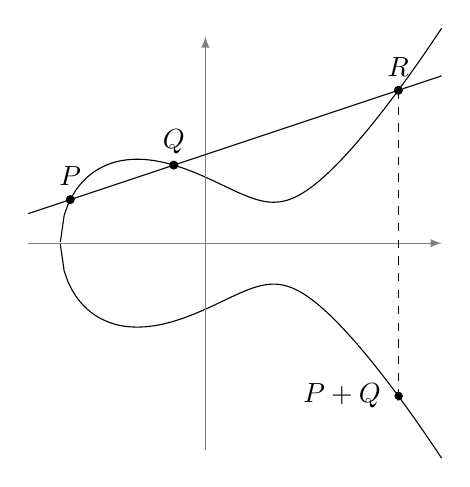
\begin{tikzpicture}[domain=-2.4566:4,samples=100,yscale=3/8,xscale=3/4]
		\draw plot (\x,{sqrt(\x*\x*\x-4*\x+5)});
		\draw plot (\x,{-sqrt(\x*\x*\x-4*\x+5)});
	
		\draw[thin,gray,-latex] (0,-7) -- (0,7);
		\draw[thin,gray,-latex] (-3,0) -- (4,0);
	
		\draw (-3,1) -- (4,8/3+3);
		\begin{scope}[every node/.style={draw,circle,inner sep=1pt,fill},cm={1,2/3,0,0,(0,3)}]
			\node at (-2.287980,0) {};
			\node at (-0.535051,0) {};
			\node at (3.267475,0) {};
		\end{scope}
		\begin{scope}[every node/.style={yshift=0.3cm},cm={1,2/3,0,0,(0,3)}]
			\node at (-2.287980,0) {$P$};
			\node at (-0.535051,0) {$Q$};
			\node at (3.267475,0) {$R$};
		\end{scope}
	
		\draw[dashed] (3.267475,3.267475*2/3+3) -- (3.267475,-3.267475*2/3-3) 
			node[draw,circle,inner sep=1pt,fill] {}
			node[xshift=-0.1cm,anchor=east] {$P+Q$};
	\end{tikzpicture}
	\hfill
	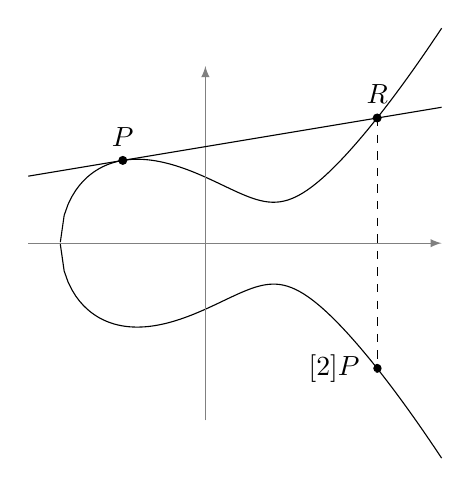
\begin{tikzpicture}[domain=-2.4566:4,samples=100,yscale=3/8,xscale=3/4]
		\draw plot (\x,{sqrt(\x*\x*\x-4*\x+5)});
		\draw plot (\x,{-sqrt(\x*\x*\x-4*\x+5)});
		
		\draw[thin,gray,-latex] (0,-6) -- (0,6);
		\draw[thin,gray,-latex] (-3,0) -- (4,0);
	
		\def\c{3.269524}
		\def\P{-1.398674}
		\def\R{2.908459}
		\draw (-3,-1+\c) -- (4,4/3+\c);
		\begin{scope}[every node/.style={draw,circle,inner sep=1pt,fill}, cm={1,1/3,0,0,(0,3.269524)}]
			\node at (\P,0) {};
			\node at (\R,0) {};
		\end{scope}
		\begin{scope}[every node/.style={yshift=0.3cm},cm={1,1/3,0,0,(0,3.269524)}]
			\node at (\P,0) {$P$};
			\node at (\R,0) {$R$};
		\end{scope}
	
		\draw[dashed] (\R,\R/3+\c) -- (\R,-\R/3-\c) 
			node[draw,circle,inner sep=1pt,fill] {}
			node[xshift=-0.1cm,anchor=east] {$[2]P$};
	\end{tikzpicture}

		\hfill
		\strut
	
	\end{center}
	
	\caption{An elliptic curve defined over $\mathbb{R}$, and the geometric
		representation of its group law.}
	\label{fig:weierstrass}
\end{figure}
\end{frame}

\begin{frame}
\frametitle{Supersingular Elliptic Curves}
	\begin{definition}
		For every $n$, we have a multiplication map 
			\[[n]: E \to E\]
			\[ P \mapsto \underbrace{P \oplus \cdots \oplus P}_{n \ \text{times}}. \]
		Its kernel is denoted by $E[n]$ and is called the $n$-torsion subgroup of $E$. Then one can show that for any $r \geq 1$:
			\[ E[p^r](\bar{K}) \simeq
				\begin{cases}
					{0} \\
					\mathbb{Z}/p^r\mathbb{Z}
				\end{cases} \]
		In the first case, $E$ is called \alert{supersingular}. Otherwise, it is called ordinary.
	\end{definition}
\end{frame}

\section{Isogeny Graphs}

\begin{frame}
\frametitle{Isogenies}
	\begin{definition}
		Let $E_1$ and $E_2$ be elliptic curves defined over a finite field $\mathbb{F}_q$ of characteristic $p$. An \alert{isogeny} $\phi: E_1 \to E_2$ defined over $\mathbb{F}_q$ is a non-constant morphism that maps the identity into the identity (and this a is group homomorphism).
	\end{definition}
	
	\begin{theorem}[Sato-Tate]
		Two elliptic curves $E_1$ and $E_2$ are isogenous over $\mathbb{F}_q$ if and only if $\#E_1(\mathbb{F}_q) = \#E_2(\mathbb{F}_q)$. 
	\end{theorem}

\end{frame}
\begin{frame}
\frametitle{Isogenies}
	\begin{itemize}
		\item Curves in the same isogeny class are either all supersingular or all ordinary.
		
		\item The degree of an isogeny $\phi$ is the degree of $\phi$ as a morphism. An isogeny of degree $\ell$ is called $\ell$-isogeny.
		
		\item \alert{An isogeny could be identified with its kernel}.Given a subgroup $G$ of $E$, we can use Velu's formulas to compute an isogeny $\phi: E_1 \to E_2$ with kernel $G$ and such that $E_2 \simeq E_1/G$.
	\end{itemize}
\end{frame}

\begin{frame}
\frametitle{Isogeny graphs}

	\begin{definition}
		Let $E$ be an elliptic curve over a field $K$. Let $S \subseteq \mathbb{N}$ be a finite set of primes. Define
			\[X_{E, K, S} \]
		to be the graph with vertex set being the $K$-isogeny class of $E$. Vertices are typically labelled by $j(E)$. There is an edge $(j(E_1), j(E_2))$ labelled by $\ell$ for each equivalence class of $\ell$-isogenies from $E_1$ to $E_2$ defined over $K$ for some $\ell \in S$. This graph is called \alert{isogeny graph}.
	\end{definition}

	Supersingular isogeny graph is always
		\begin{itemize}
			\item connected;
			\item $\ell + 1$-regular, where $\ell$ is isogeny degree and $S = \{\ell\}$.
		\end{itemize}
\end{frame}

\begin{frame}
\begin{figure}[h]
	\begin{center}
		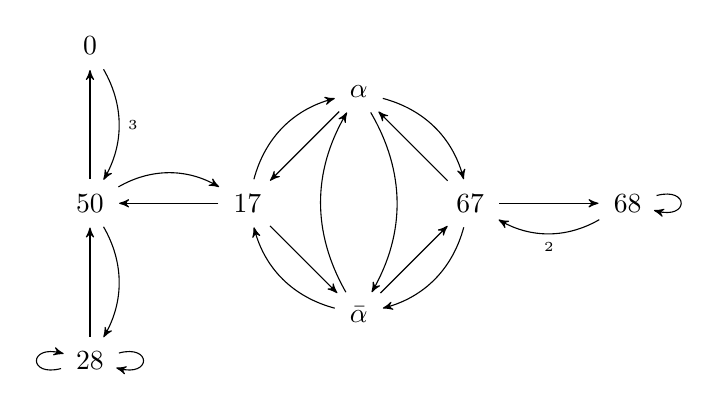
\begin{tikzpicture}[->, shorten >=2pt, shorten <=2pt, >=stealth', node distance = 2cm]
		
		\node (1) {$17$};
		\node (2) [above right of=1] {$\alpha$};
		\node (3) [below right of=1] {$\bar{\alpha}$};
		\node (4) [below right of=2] {$67$};
		\node (5) [right of=4] {$68$};
		\node (6) [left of=1] {$50$};
		\node (7) [below of=6] {$28$};
		\node (8) [above of=6] {$0$};
		
		\path
		(1) edge [bend left] (2)
		(1) edge (3)
		(1) edge (6)
		
		(2) edge (1)
		(2) edge [bend left] (3)
		(2) edge [bend left] (4)
		
		(3) edge [bend left] (1)
		(3) edge [bend left] (2)
		(3) edge (4)
		
		(4) edge (2)
		(4) edge [bend left] (3)
		(4) edge (5)
		
		(5) edge [bend left] node[below]{\tiny{$2$}} (4)
		(5) edge [loop right] (5)
		
		(6) edge [bend left] (1)
		(6) edge [bend left] (7)
		(6) edge (8)
		
		(7) edge (6)
		(7) edge [loop left] (7)
		(7) edge [loop right] (7)
		
		(8) edge [bend left] node[right]{\tiny{$3$}} (6);
		
		\end{tikzpicture}
	\end{center}
	\caption{Supersingular Isogeny Graph $X_{\bar{\mathbb{F}}_{83}, 2}$}\label{SIG83.figure}
\end{figure}

\end{frame}

\section{Diffie-Hellman Key Exchange Protocol}
\subsection{Classic Diffie-Hellman}

\begin{frame}
\frametitle{Classic Diffie-Hellman}

\begin{figure}
	\centering
	\begin{tabular}{l *{2}{p{17ex}<{\centering}}}
		\hline
		Public parameters   & \multicolumn{2}{l}{A prime $p$, $p-1$ has large prime cofactor.}\\
							& \multicolumn{2}{l}{A multiplicative generator $g \in (\mathbb{Z}/p\mathbb{Z})^{\ast}$.}\\
		\hline
							& {\bf Alice} & {\bf Bob}\\
		\hline
		Pick random secret & $0 < a < p - 1$ & $0 < b < p - 1$\\
		Compute public data & $A = g^a$ & $B = g^b$\\
		Exchange data &  \hfill $A \longrightarrow$ & $\longleftarrow B$ \hfill\strut \\
		Compute shared secret & $S = B^a$ & $S = A^b$
	\end{tabular}
\end{figure}
	
	\begin{itemize}
		\item The protocol can be generalized by replacing the multiplicative group $(\mathbb{Z}/p\mathbb{Z})^{\ast}$ with any other cyclic group $G = \langle g \rangle$.
	\end{itemize}
\end{frame}

\begin{frame}
\frametitle{Security of DH}

	\begin{definition}[Discrete logarithm problem]
		Let $G$ be a cyclic group generated by an element $g$. For any element $A \in G$, find the \alert{dicrete logarithm of $A$ in base $g$}, denoted $\log_g(A)$, as the unique integer in the interval $[0, \#G[$ such that
			\[ g^{\log_g(A)} = A. \] 
	\end{definition}

	We know several algorithms to compute discrete logarithms:
	\begin{itemize}
		\item in \emph{generic} group $G$ that require $O(\sqrt{q}))$ computational steps, where $q$ is the largest prime divisor of $\#G \implies G$ is usually chosen such that $\log_2q \simeq 256$;
		
		\item in group $G = (\mathbb{Z}/p\mathbb{Z})^{\ast}$ of complexity better than $O(\sqrt{\#G})$.
	\end{itemize}
\end{frame}

\subsection{Elliptic Curve Diffie-Hellman}

\begin{frame}
\frametitle{Elliptic Curve Diffie-Hellman}

	\begin{figure}
		\centering
		\begin{tabular}{l *{2}{p{17ex}<{\centering}}}
			\hline
			Public parameters   & \multicolumn{2}{l}{Finite field $\mathbb{F}_p$, with $\log_2p \simeq 256$,}\\
								& \multicolumn{2}{l}{Elliptic curve $E/\mathbb{F}_p$,  $\#E(\mathbb{F}_p)$ is prime,}\\
								& \multicolumn{2}{l}{A generator $P$ of $E(\mathbb{F}_p)$.}\\
			\hline
								& {\bf Alice} & {\bf Bob}\\
			\hline
			Pick random secret  & $0<a<\#E(\mathbb{F}_p)$ & $0<b<\#E(\mathbb{F}_p)$\\
			Compute public data & $A = [a]P$ & $B = [b]P$\\
			Exchange data &  \hfill $A \longrightarrow$ & $\longleftarrow B$ \hfill\strut \\
			Compute shared secret & $S = [a]B$ & $S = [b]A$
		\end{tabular}
	\end{figure}

\end{frame}

%\begin{frame}
%\frametitle{Security of ECDH}
%\end{frame}

\subsection{Supersingular Isogeny Diffie-Hellman}

\begin{frame}
\frametitle{Background}
	Let $G = (V, E)$ be an undirected graph, where $V = \{ v_i | i \in I\}$ is the set of vertices, and $E$ is the set of edges. A \alert{random walk} of length $i$ is a path $v_1 \to \cdots \to v_i$, defined by the random process that selects $v_i$ uniformly at random among the neighbours of $v_{i-1}$.
	 
	Why do we use \alert{supersingular} isogenies?
	\begin{itemize}
		\item One isogeny degree is sufficient to obtain an expander graph $\sim$ graph with short diameter and rapidly mixing walks $\implies$we can construct more efficient protocols.
	
		\item  There is no action of an abelian group on them $\implies$ harder to use quantum computers to speed up the supersingular isogeny path problem.
	\end{itemize}
\end{frame}

\begin{frame}
\frametitle{Idea of SIDH}

	\begin{itemize}
		\item \underline{Secrets:} Alice and Bob take secret random walks in two \alert{distinct} isogeny graphs on \alert{the same vertex set}. Alice's walk has length $\varepsilon_A$ and Bob's has length $\varepsilon_B$.
		
			\begin{itemize}
				\item \emph{On practice}, we choose a large prime $p$ and small primes $\ell_A$ and $\ell_B$. The vertex set is elliptic curves $j$-invariant over $\mathbb{F}_{p^2}$. Alice's graph consists of $\ell_A$-isogenies, Bob's - of $\ell_B$-isogenies.
			\end{itemize}
	
		\item \underline{Key idea:} A walk of length $\varepsilon_A$ in the $\ell_A$-isogeny graph corresponds to a kernel of a size $\ell_A^{\varepsilon_A}$, and this kernel is cyclic $\iff$ the walk does not backtrack.
			\begin{itemize}
				\item \emph{On practice}, choosing a secret walk of length $\varepsilon_A$ is equivalent to choosing a secret cyclic subgroup $\langle A \rangle \subset E[\ell_A^{\varepsilon_A}]$.
			\end{itemize}
		\item \underline{Shared secret:} A subgroup $\langle A \rangle + \langle B \rangle = \langle A, B \rangle$  defines an isogeny to $E/\langle A, B \rangle$. Since we choose $\ell_A \neq \ell_B$, the group $\langle A, B \rangle$ is cyclic of order $\ell_A^{\varepsilon_A} \ell_B^{\varepsilon_B}$.	
	\end{itemize}
\end{frame}

\begin{frame}
\begin{figure}[h]
	\centering
	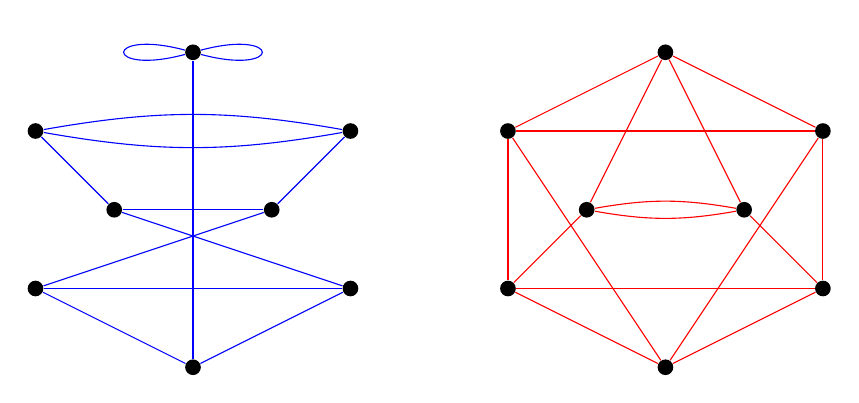
\begin{tikzpicture}
	\def\graph{
		\begin{scope}[every node/.style={fill,black,circle,inner sep=2pt}]
		\node at (0,0)  (1){};
		\node at (0,4) (20){};
		\node at (2,1)  (16z){};
		\node at (-2,1)  (81z){};
		\node at (-1,2) (77z){};
		\node at (1,2)  (20z){};
		\node at (-2,3)  (85z){};
		\node at (2,3)  (12z){};
		\end{scope}
	}
	
	\graph
	\begin{scope}[blue,every loop/.style={looseness=50}]
	\path (1) edge (20) edge (16z) edge (81z);
	\path (20) edge[loop left] (20) edge[loop right] (20);
	\path (16z) edge (81z) edge (77z);
	\path (81z) edge (20z);
	\path (77z) edge (20z) edge (85z);
	\path (20z) edge (12z);
	\path (12z) edge[bend right=10] (85z) edge[bend left=10] (85z);
	\end{scope}
	
	\begin{scope}[xshift=6cm]
	\graph
	\begin{scope}[red]
	\path (1) edge (85z) edge (81z) edge (12z) edge (16z);
	\path (20) edge (85z) edge (77z) edge (20z) edge (12z);
	\path (81z) edge (85z) edge (77z) edge (16z);
	\path (85z) edge (12z);
	\path (12z) edge (16z);
	\path (16z) edge (20z);
	\path (20z) edge[bend right=10] (77z) edge[bend left=10] (77z);
	\end{scope}
	\end{scope}
	\end{tikzpicture}
	\caption{Supersingular isogeny graphs of degree 2 (left, blue) and 3
		(right, red) on $\mathbb{F}_{97^2}$.}
	\label{SIG97-2-3:figure}
\end{figure}

\end{frame}

\begin{frame}
\frametitle{Illustration of SIDH}
\begin{figure}
	\centering
	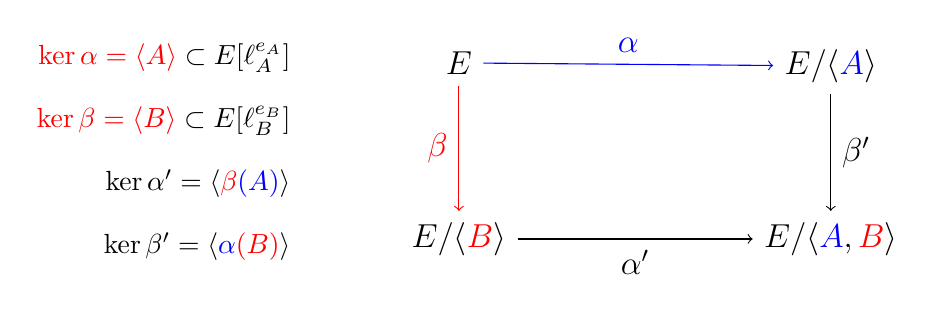
\begin{tikzpicture}
	
	\begin{scope}
	\draw (0,1.2) node[anchor=east] {$\textcolor{red}{\ker \alpha=\langle A\rangle} \subset E[\ell_A^{e_A}]$};
	
	\draw (0,0.4) node[anchor=east] {$\textcolor{red}{\ker \beta=\langle B\rangle} \subset E[\ell_B^{e_B}]$};
	
	\draw (0,-0.4) node[anchor=east] {$\ker \alpha' = \langle\textcolor{red}{\beta}\textcolor{blue}{(A)}\rangle$};
	
	\draw (0,-1.2) node[anchor=east] {$\ker \beta' = \langle\textcolor{blue}{\alpha}\textcolor{red}{(B)}\rangle$};
	\end{scope}
	
	\begin{scope}[xshift=4.5cm]
	\large
	\node[matrix of nodes, ampersand replacement=\&, column sep=3cm, row sep=1.5cm] (diagram) {
		|(E)| $E$ \& |(Es)| $E/\langle\textcolor{blue}{A}\rangle$ \\
		|(Ep)| {$E/\langle\textcolor{red}{B}\rangle$} \& |(Eps)| {$E/\langle\textcolor{blue}{A},\textcolor{red}{B}\rangle$}\\
	};
	
	\path[->,blue] (E) edge node[auto] {$\alpha$} (Es);
	
	\path[->] (Ep) edge node[auto,swap] {$\alpha'$} (Eps);
	
	\path[->,red] (E) edge node[auto,swap] {$\beta$} (Ep);
	
	\path[->] (Es) edge node[auto] {$\beta'$} (Eps);
	\end{scope}
	\end{tikzpicture}
	\caption{Commutative isogeny diagram constructed from Alice's and
		Bob's secrets. Quantities known to Alice are drawn in blue, those known to Bob are drawn in red.} \label{SIDH-diagram:figure}
\end{figure}
\end{frame}

\begin{frame}
\frametitle{The problems we face}
	\begin{enumerate}
		\item The points of $\langle A \rangle$ (or $\langle B \rangle$) may not be rational.
		
		\item The diagram on previous slide shows no way how Alice and Bob could compute shared secret $E/\langle A, B \rangle$ without revealing their secrets.
	\end{enumerate}
\end{frame}

\begin{frame}
\frametitle{Solution of the 1st problem}

	\begin{itemize}
		\item In case of \alert{supersingular} curves, we can control the group structure. It turns out that as we are dealing with the field $\mathbb{F}_{p^2}$ then
			\[ E(\mathbb{F}_{p^2}) \simeq (\mathbb{Z}/(p \pm 1)\mathbb{Z})^2. \]
			
		\item We choose $p$ so that $E(\mathbb{F}_{p^2})$ contains two large subgroups $E[\ell_A^{\varepsilon_A}]$ and $E[\ell_B^{\varepsilon_B}]$ of coprime order.
		
		\item Once subgroups are fixed, we look for a prime of the form $p = \ell_A^{\varepsilon_A} \ell_B^{\varepsilon_B}f \mp 1$, where $f$ is a small cofactor.
			\begin{itemize}
				\item \emph{On practice}, we can choose $f = 1$.
			\end{itemize}
	\end{itemize}
	$\implies$ $E(\mathbb{F}_{p^2})$ contains $\ell_A^{\varepsilon_A - 1}(\ell_A + 1)$  cyclic subgroups of order $\ell_A^{\varepsilon_A}$, each defining a distinct isogeny; $\implies$ a single point $A \in E(\mathbb{F}_q)$ is enough to represent an isogeny walk of length $\varepsilon_A$.
	
\end{frame}

\begin{frame}
\frametitle{Solution of the 2nd problem}
	Solution is to publish some additional data.
	
	\begin{itemize}
		\item They have publicly agreed on a prime $p$ and a supersingular curve $E$ such that
			\[ E(\mathbb{F}_{p^2}) \simeq (\mathbb{Z}/\ell_A^{\varepsilon_A}\mathbb{Z})^2 \oplus (\mathbb{Z}/\ell_B^{\varepsilon_B}\mathbb{Z})^2 \oplus (\mathbb{Z}/f\mathbb{Z})^2. \]
		
		\item They fix public bases of their respective torsion groups:
		\[ E[\ell_A^{\varepsilon_A}] = \langle P_A, Q_A \rangle, \]
		\[ E[\ell_B^{\varepsilon_B}] = \langle P_B, Q_B \rangle. \]
		
		\item They choose random secret subgroups defined as follows
		\[ \langle A \rangle = \langle [m_A]P_A + [n_A]Q_A \rangle \subset E[\ell_A^{\varepsilon_A}], \]
		\[ \langle B \rangle = \langle [m_B]P_B +[n_B]Q_B \rangle \subset E[\ell_B^{\varepsilon_B}]. \]
		
		
	\end{itemize}

\end{frame}

\begin{frame}
\frametitle{Solution of the 2nd problem}
	\begin{itemize}
		
		\item After computing secret isogenies $\alpha$ and $\beta$, Alice publishes $\alpha(P_B)$ and $\alpha(Q_B)$ and Bob publishes $\beta(P_A)$ and $\beta(Q_A)$.
		
		\item Alice computes $\beta(A) = [m_A]\beta(P_A) + [n_A]\beta(Q_A)$ and Bob computes $\alpha(B) = [m_B]\alpha(P_B) + [n_B]\alpha(Q_B)$.
		
		\item They compute isogenies $\alpha', \beta'$, whose kernels are generated respectively by $\langle \beta(A) \rangle$ and $\langle \alpha(A) \rangle$
		$\implies$ They compute the shared secret $E/\langle A, B \rangle$.
	\end{itemize}
\end{frame}

\begin{frame}

\begin{figure}

	\begin{tabular}{l *{2}{p{23ex}<{\centering}}}
		\hline
		Parameters & \multicolumn{2}{l}{Primes $\ell_A,\ell_B, p=\ell_A^{\varepsilon_A}\ell_B^{\varepsilon_B}f \mp 1$,}\\
		& \multicolumn{2}{l}{A supersingular curve $E$ over $\mathbb{F}_{p^2}$ of order $(p \pm 1)^2$,}\\
		& \multicolumn{2}{l}{A basis $\langle P_A,Q_A \rangle$ of $E[\ell_A^{\varepsilon_A}]$,}\\
		& \multicolumn{2}{l}{A basis $\langle P_B,Q_B \rangle$ of $E[\ell_B^{\varepsilon_B_B}]$,}\\
		\hline
		& {\bf Alice} & {\bf Bob}\\
		\hline
		Random secret & $A=[m_A]P_A+[n_A]Q_A$ & $B=[m_B]P_B+[n_B]Q_B$\\[1ex]
		Secret isogeny & $\alpha:E\to E_A=E/\langle A \rangle $ & $\beta:E\to E_B=E/\langle B \rangle$\\[1ex]
		Exchange data &  \hfill $E_A,\alpha(P_B),\alpha(Q_B) \longrightarrow$ & $\longleftarrow E_B,\beta(P_A),\beta(Q_A)$ \hfill\strut \\[1ex]
		Shared secret & $E/\langle A,B \rangle = E_B/\langle \beta(A) \rangle$ & $E/\langle A,B \rangle = E_A/ \langle \alpha(B)\rangle$
	\end{tabular}
	
	\caption{Supersingular Isogeny Diffie-Hellman key exchange protocol.}
	\label{fig:sidh-prot}
\end{figure}

\end{frame}

\begin{frame}
\frametitle{Security of SIDH}
	\begin{definition}[Supersingular Decision Diffie-Hellman]
		%Let $E, \ell_A, \ell_B, \varepsilon_A, \varepsilon_B, P_A, Q_A, P_B, Q_B$ be the parameters of a SIDH protocol.
		
		Given a tuple sampled with probability  $1/2$ from one of the following two distributions:
		\begin{enumerate}
			\item $(E/\langle A \rangle, \phi(P_B), \phi(Q_B). E/\langle B \rangle, \psi(P_A), \psi(Q_A), e/\langle A, B \rangle)$, where
			
			\begin{itemize}
				\item $A \in E$ is a uniformly random point of order $\ell_A^{\varepsilon_A}$,
				
				\item $B \in E$ is a uniformly random point of order $\ell_B^{\varepsilon_B}$,
				
				\item $\phi: E \to E/\langle A \rangle$ is the isogeny of kernel $\langle A \rangle$, and
				
				\item $\psi: E \to E/\langle B \rangle$ is the isogeny of kernel $\langle B \rangle$;
			\end{itemize}
			
			\item $(E/\langle A \rangle, \phi(P_B), \phi(Q_B), E/\langle	B \rangle, \psi(P_A), \psi(Q_A), E/\langle C \rangle)$, where $A, B, \phi, \psi$ are as above, and where $C \in E$ is a uniformly random point of order $\ell_A^{\varepsilon_A}\ell_B^{\varepsilon_B}$;
		\end{enumerate}
		determine from which distribution the tuple is sampled.
	\end{definition}
\end{frame}

\begin{frame}
\frametitle{Security of SIDH}
	\begin{itemize}
		\item The best known algorithms for SSDDH have \alert{exponential complexity}, even on a quantum computer.
		
		\item Although there is no efficient algorithms to solve SSDDH at the time of writing, several polynomial-time attacks have appeared  against variations of SIDH.
	\end{itemize}
\end{frame}

\begin{frame}
\frametitle{Analogues between DH instantiations}
\begin{figure}[h]
	\begin{center}
		\begin{tabular}{| m{2.3cm} | m{2.5cm} m{2.5cm} m{2.5cm} |}
			\hline
			~ & DH & ECDH & SIDH\\
			\hline
			\textbf{Element}s & Integers $g$ modulo prime & Points $P$ in elliptic curve group & Curves $E$ in isogeny class\\
			\hline
			\textbf{Secrets} & Exponents $x$ & scalars $k$ & isogenies $\phi$ \\
			\hline
			\textbf{Computations} & $(g, x) \to g^x$ & $(P, k) to [k]P$ & $(E, \phi) \to \phi(E)$\\
			\hline
			\textbf{Hard problem} & Given $g, g^x$. Find $x$ & Given $P,[k]P$. Find $k$ & Given $E, \phi(E)$. Find $\phi$\\
			\hline 
		\end{tabular}
	\end{center}
	\caption{Analogues between DH instantiations}\label{DH-Analogues-table:figure}
\end{figure}
\end{frame}

\begin{frame}
	\begin{center}
		\Huge{Thank you!}
	\end{center}
\end{frame}
\end{document}
